\documentclass[10pt, a4paper]{article}

%==============================================================
%Paketi
%==============================================================
\usepackage[slovene]{babel}
\usepackage[utf8]{inputenc} %za šumnike
\usepackage{lmodern}
\usepackage[T1]{fontenc}
\usepackage{eurosym}

\usepackage{graphicx}
\graphicspath{{./slike/}{./program_slike/}{./primer_slike/}}

%==============================================================
%Dokument
%==============================================================
\begin{document}

\begin{center}
\Huge \textbf{Naslov Skupina 19: Graffiti conjecture 232} \\
\medskip
\Large Urban Merhar, Martin Kokošinek\\
\end{center}

\section{Navodilo}
Računalniško generirana domneva trdi: Če je $G$ enostaven povezan graf, potem
\begin{center}
 $2\gamma_{t}(G) \geq rad(G) + ecc(B)$.
\end{center}
 
Preveri domnevo na različne načine za male in velike grafe. Z uporabo populacijske metahevristike, preveri domnevo v upanju, da jo ovržeš.

\medskip
Nekaj pripomb:

\begin{enumerate}
\item $ecc(v)$ je $ekscentričnost$ od vozlišča $v$. Ekscentričnost od $v$ je razdalja do najbolj oddaljenega vozlišča od vozlišča $v$, i.e., $ max\{d(v,u): u$ je vozlišče na grafu $\}$.
\item $rad(G)$ je $radij$ grafa, t.j., minimum vseh ekscentričnosti vozlišč grafa $G$.
\item $B$ je $obrobje$ grafa $G$, t.j., množica vozlišč z maksimalno ekscentričnostjo.
\item $ecc(S)$ je $ekscentričnost$ množice vozlišč $S$. Definirana je kot: Naj bo $S$ podmnožica množice vozlišč $V$. Razdalja med vozliščem $v$ in množico $S$, definirajmo kot razdaljo od $v$ do najbližjega volišča v $S$. $ecc(S)$ je maksimum razadalj od vozlišča v $V\backslash S$ do množice $S$.
\end{enumerate}


\section{Kratek opis}
$Computer\ generated\ conjectures$ so računalniško ustvarjene domneve. $Graffiti$ je računalniški program, ki generira te matematične domneve oziroma odprte probleme. Računalniši program $Graffiti$ je ustvaril $Siemion\ Fajtlowicz$.\\

V najinem projektu pri predmetu Finančni praktikum si bova ogledala $Graffiti$ $conjecture$ $232$, ki jo bova testirala za majhne in velike grafe v upanju, da najdeva protiprimer. Ideja je, da enačbo zapiševa v programskem jeziku $Sage$ in generirava naključne grafe. Na vsakem od teh grafov pa predpostavko testirava.\\


Že vgrajene funkcije, ki jih bova uporabila v programu:
\begin{enumerate}
	\item $dominating\_ set(total=True, value\_ only=True)$ vrne najmanjšo dominirajočo množico na grafu $G$.
	\item $radius()$ vrne radij grafa $G$.
	\item $eccentricity()$ vrne ekscentričnost vozlišča $v$.
	\item $periphery()$ vrne množico vozlišč iz obrobja grafa $G$.
\end{enumerate}

\subsection{Razlaga pojmov}
\begin{itemize}
\item Dominirajoča Množica $D$: $D$ je množica, kjer je vsako vozlišče iz $G \backslash D$ sosed nekega vozlišča iz $D$.
\item Totalno Dominirajoča množica (TDM): Dominirajoči množici $D$ dodamo pogoj, da so tudi vozlišča dominirajoče množice 
$D$ sosedi vozlišč iz $D$.
\item Totalno Dominirajoče Število (TDŠ): Moč totalno dominirajoče množice grafa $G$.
\item $\gamma_{t}(G)$ je TDŠ grafa $G$.
\end{itemize}

\subsubsection{Populacijska metahevristika}
\textbf{Hevristika} (iz Grščine: 'najdem, odkrijem'): V računalništvu in matematični optimizaciji je visoko-nivojski način reševanja problemov, ko so klasični postopki prepočasni oziroma, ko klasične metode ne vrnejo točnih rezultatov. V zameno za polnost, optimalnost, natančnost, raje pridobimo na časovni zahtevnosti. \\
\textbf{Meta-hevristika} (meta iz Grščine: 'za, onstran') oziroma v prevodu Izčrpna-hevristika: Metahevristika vzame množico rešitev, ki je prevelika za analizo in s pomočjo določenih predpostavk glede optimizacije vrne zadovoljivo rešitev. Ta ni nujno globalno optimalna. \\
\textbf{Populacijska metahevristika}: Ohranjamo večje število kandidatov za rešitev in jih izboljšujemo s pomočjo populacijsih karakteristik. Primer je particle swarm optimization (PSO).

\section{Plan dela}
Zapisati učinkovit algoritem, ki bo za vsak generiran graf preveril lastnosti grafa in posledično domnevo. Za grafe, kjer  domneva ne bi držala pa nam izpiše graf in vrne vrednosti lastnosti, ki so potrebovane v domnevi.

\section{Potek dela}

Za preverjanje dane domneve sva napisala program, ki jo testira. Samo domnevo pa sva nekoliko obrnila na način, da lahko učinkovito gledava tudi njeno razliko. To sva storila z namenom da opazujeva kateri grafi so bližje temu, da bi bili lahko protiprimer domneve. Kot je vidno v spodnjem programu sva tako na grafih preverjala $2\gamma_{t}(G) - rad(G) - ecc(B) \geq 0$. Na ta način sva s pomočjo razlike $2\gamma_{t}(G) - rad(G) - ecc(B)$ ocenjevala kako blizu pride nek graf k temu, da bi bil protiprimer.

Funkcija z imenom $domneva(G)$ sprejme dan graf $G$ in na njem testira domnevo ter vrne razliko $2\gamma_{t}(G) - rad(G) - ecc(B)$, če predpostavka velja, sicer pa pove, da predpostavka ne velja.

Program je predstavljen na spodnjih slikah:

\begin{center}
\textbf{Program za preverjanje domneve}
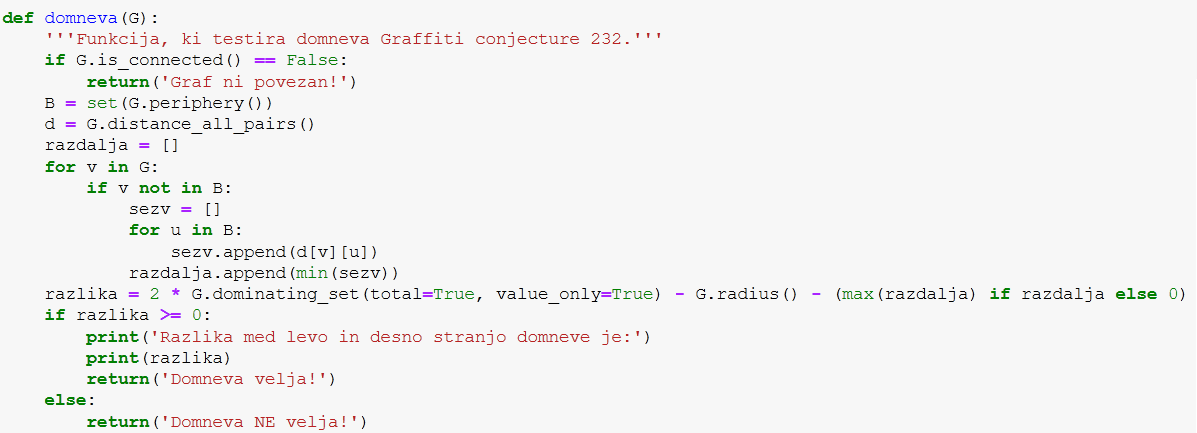
\includegraphics[width=16cm]{domneva}
\end{center}

\begin{center}
\textbf{Posamezne funkcije v programu}
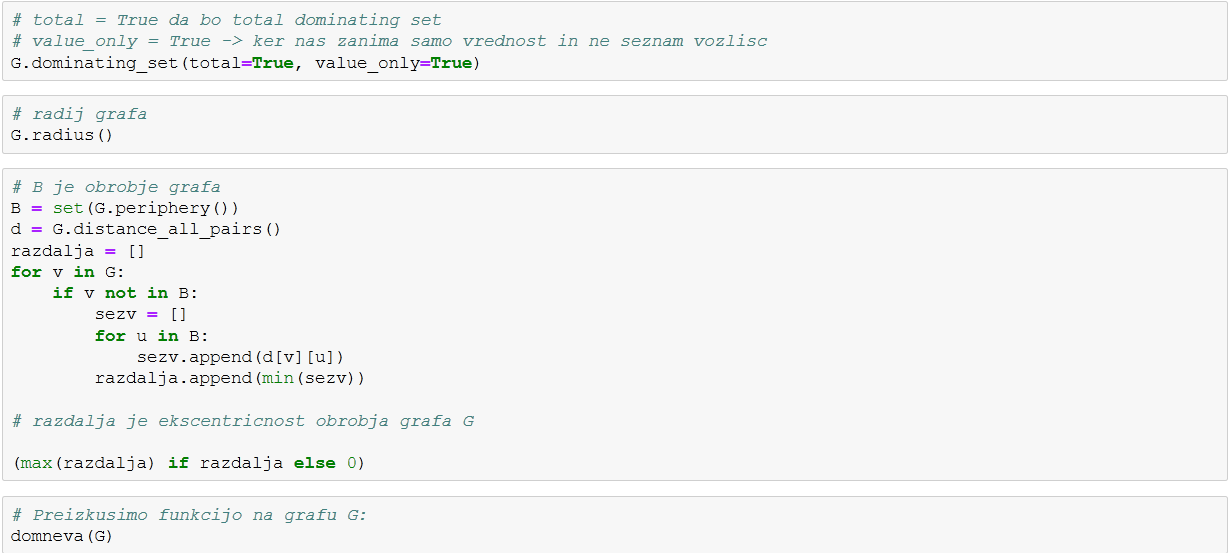
\includegraphics[width=16cm]{deli_programa}
\end{center}

\pagebreak

\section{Primer}

\begin{center}
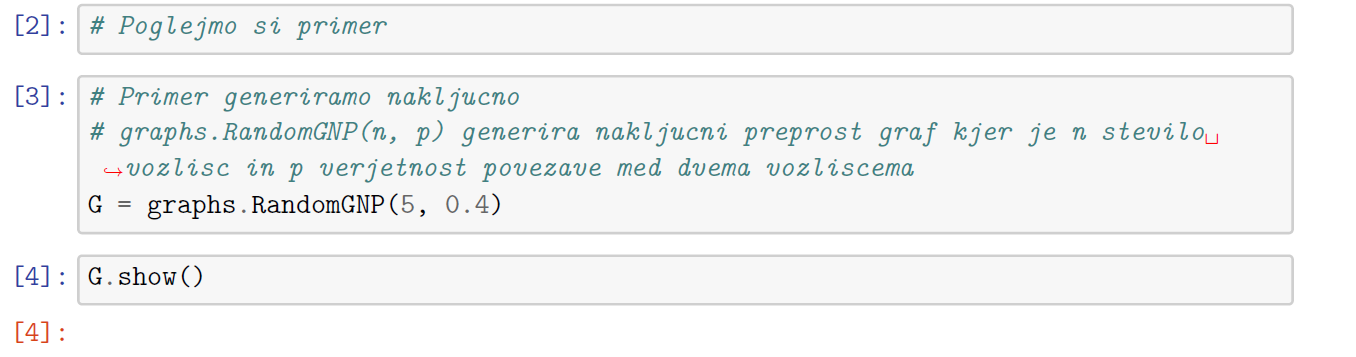
\includegraphics[width=16cm]{primer_1}
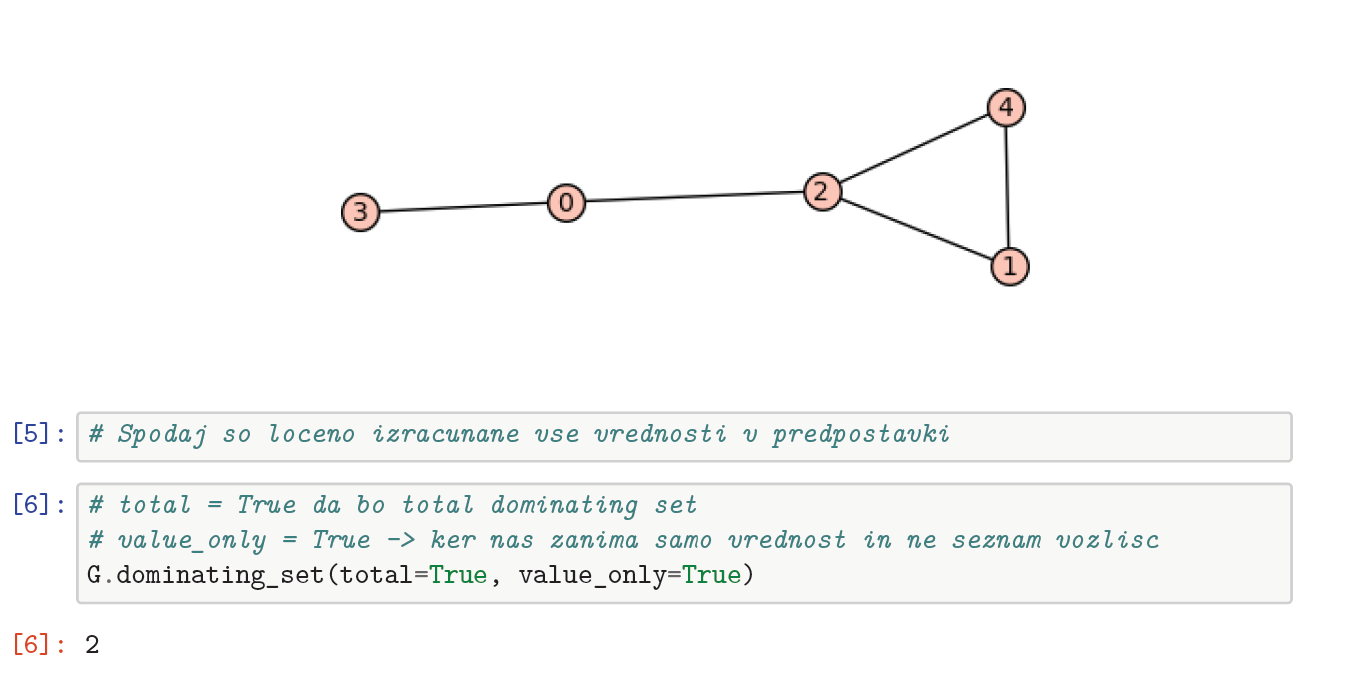
\includegraphics[width=16cm]{primer_2}
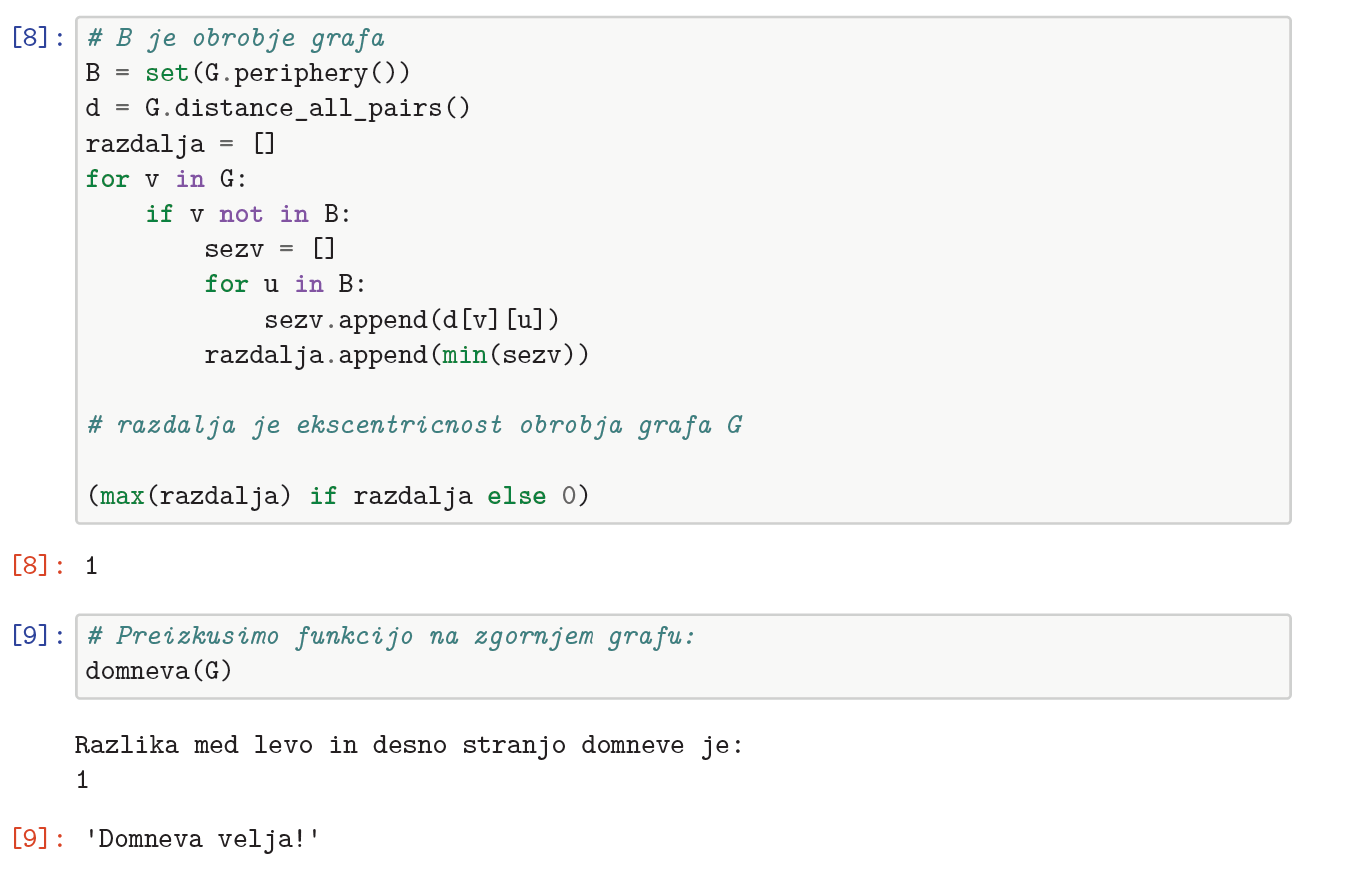
\includegraphics[width=16cm]{primer_3}
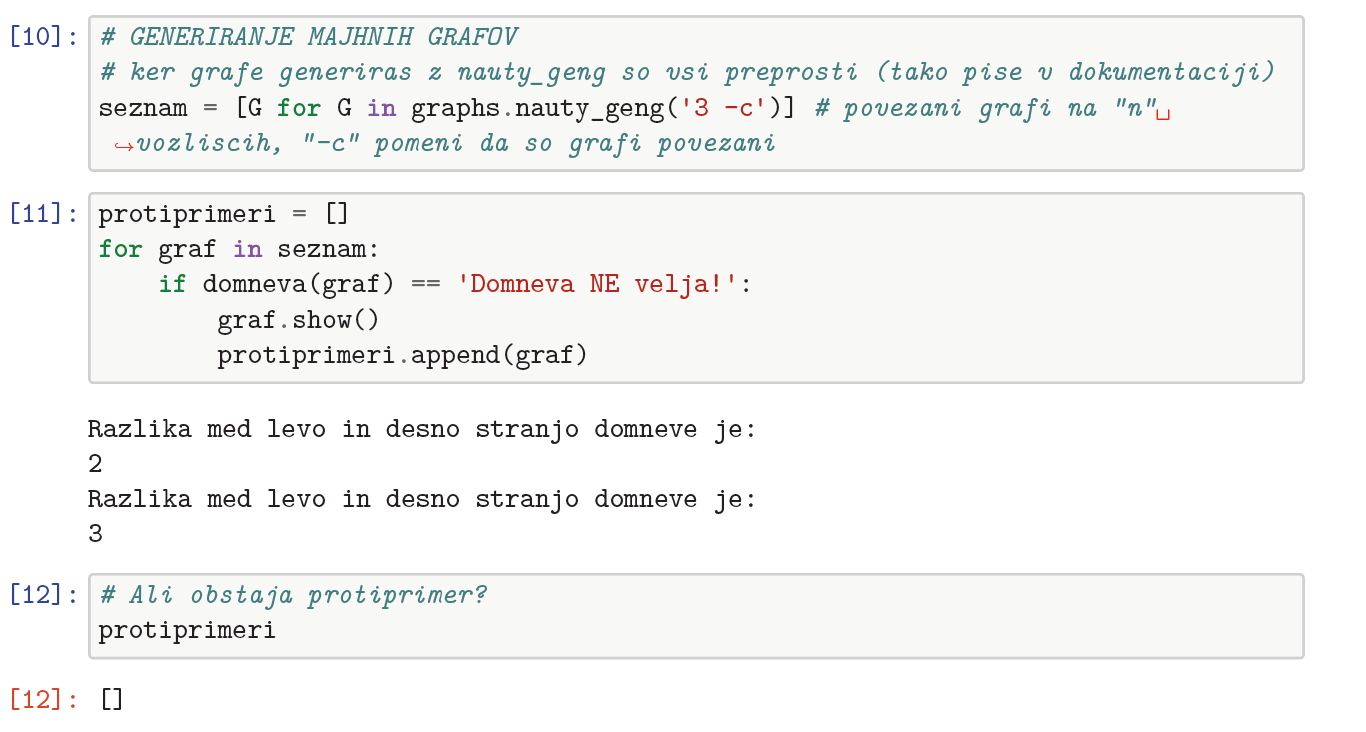
\includegraphics[width=16cm]{primer_4}
\end{center}

\section{Majhni grafi}

Majhne grafe sva v $sagu$ generirala s pomočjo funkcije $graphs.nauty\_geng('v\ -c')$. Kjer je $v$ število vozlišč grafa, $-c$ pa pomeni, da so grafi povezani. Na dovolj majhnih grafih sva generirala vse možne enostavne in povezane grafe ter na njih testirala predpostavko.

\begin{center}
\textbf{Generator malih grafov}
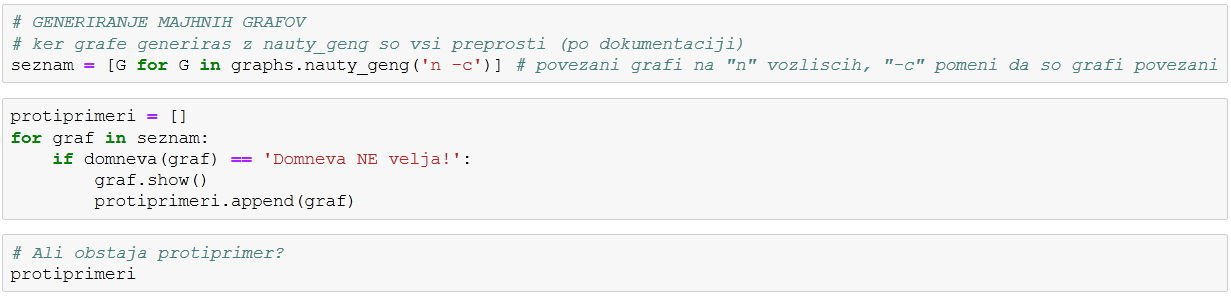
\includegraphics[width=16cm]{mali_grafi}
\end{center}

Vsi grafi so ji ustrezali, zato sva se odločila podrobneje pogledati grafe, kjer je bila razlika med levo in desno stranjo predpostavke najmanjša.

Graf na dveh vozliščih. Razlika v predpostavki je  $2\gamma_{t}(G) - rad(G) - ecc(B) = 3$.

\begin{center}
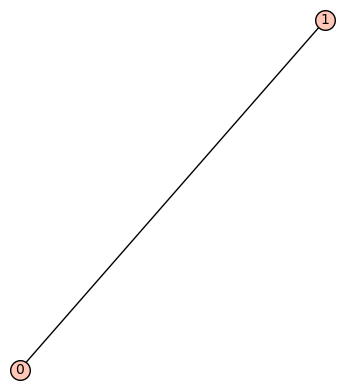
\includegraphics[height=5cm]{min_graf_2}
\end{center}

Graf na treh vozliščih. Razlika je $2$.

\begin{center}
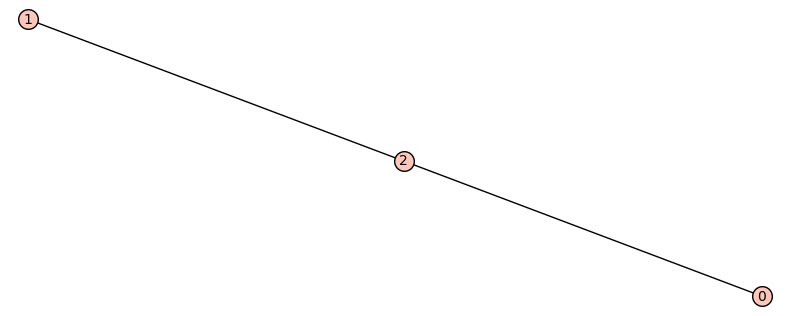
\includegraphics[height=5cm]{min_graf_3}
\end{center}

Grafi na štirih vozliščih imajo razliko predpostavke enako $1$.

\begin{center}
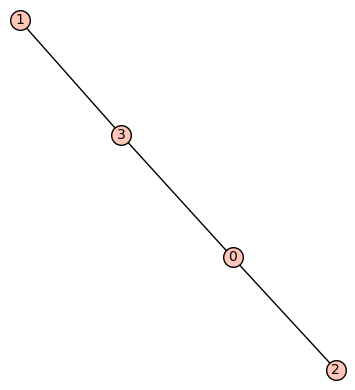
\includegraphics[height=5cm]{min_graf_4}
\end{center}

Pri grafih generiranih na petih vozliščih dobiš graf katerega razlika predpostavke je $0$. Generiranih je skupno $21$ grafov na pet vozliščih. Program testira vse te grafe v manj kot $0.2$ sekunde.

\begin{center}
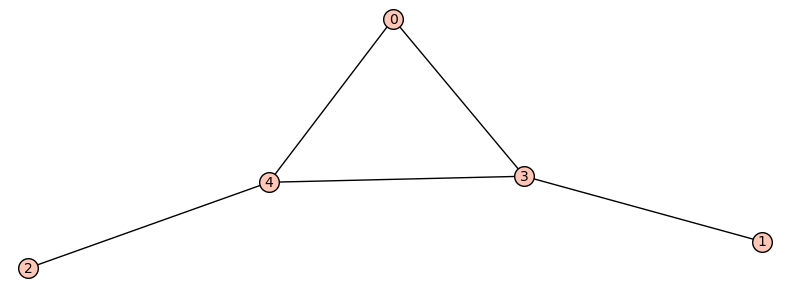
\includegraphics[height=5cm]{min_graf_5}
\end{center}

Pri grafih na šest vozliščih je razlika ponovno $0$. Od skupno $112$ vseh možnih grafov na šest vozliščih ima razliko $0$ natanko $8$ grafov. Program testira vse šestvozliščne grafe v približno $0.8$ sekunde. Spodaj je prikazanih pet primerov.

\begin{center}
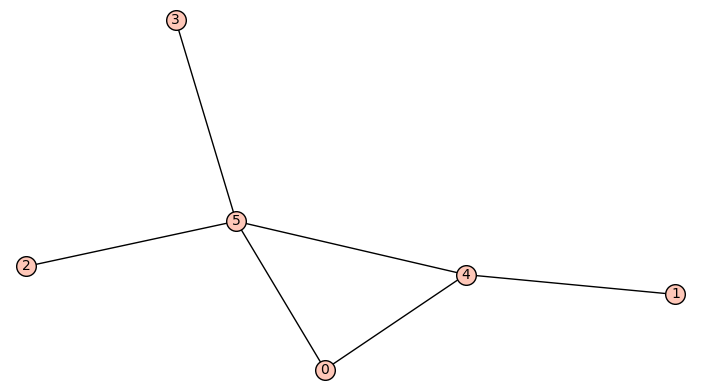
\includegraphics[height=6cm]{min_graf_6_1}
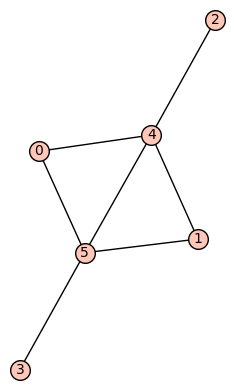
\includegraphics[height=6cm]{min_graf_6_2}
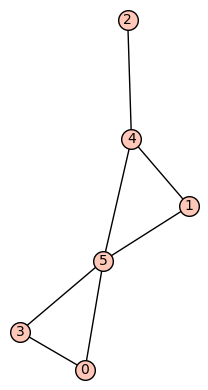
\includegraphics[height=6cm]{min_graf_6_3}
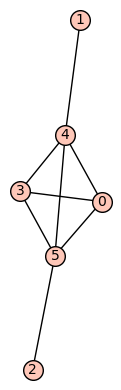
\includegraphics[height=6cm]{min_graf_6_4}
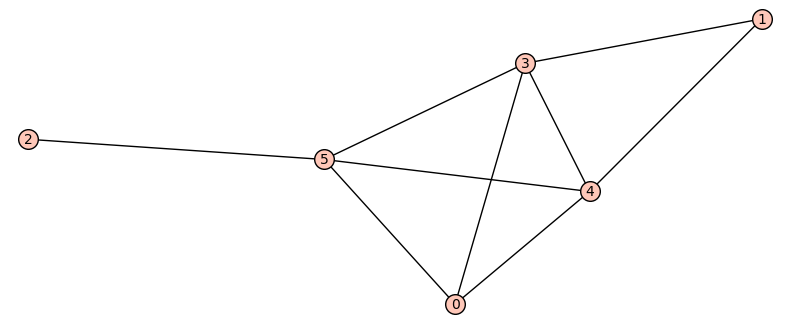
\includegraphics[height=5cm]{min_graf_6_5}
\end{center}

Za grafe na sedem vozliščih je minimalna razlika predpostavke ponovno $0$. Sedaj je možno generirati $853$ različnih grafov, razliko $0$ pa jih ima $101$. Program testira to predpostavko na vseh generiranih grafih na sedmih vozliščih v približno $3.7$ sekunde. Ponovno si poglejmo nekaj primerov teh grafov.

\begin{center}
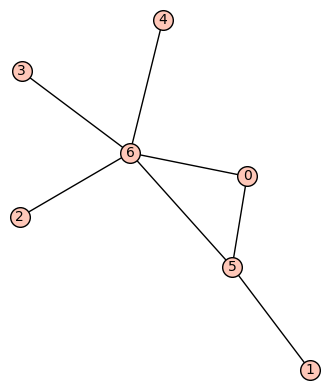
\includegraphics[height=6cm]{min_graf_7_1}
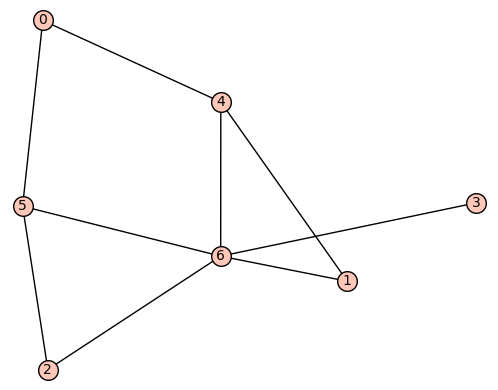
\includegraphics[height=6cm]{min_graf_7_2}
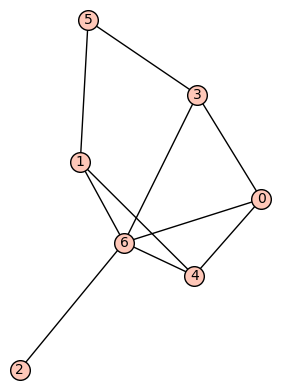
\includegraphics[height=6cm]{min_graf_7_3}
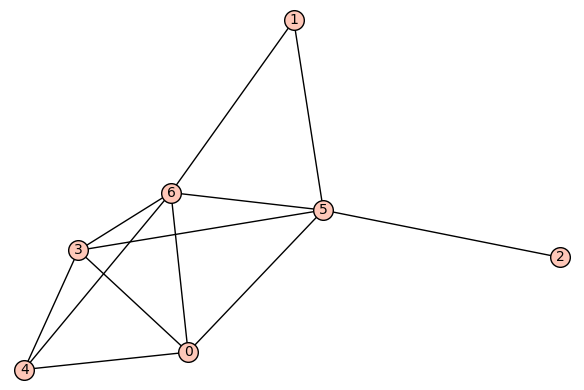
\includegraphics[height=6cm]{min_graf_7_4}
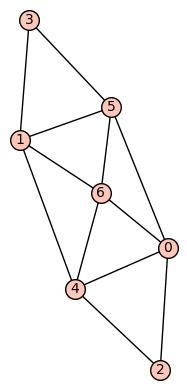
\includegraphics[height=6cm]{min_graf_7_5}
\end{center}

Grafi na osmih vozliščih imajo razliko leve in desne strani ponovno enako $0$. Zdaj generiramo že $11117$ različnih grafov in za njihovo testiranje porabimo že kar približno $40$ sekund. Grafov z osmimi vozlišči, kjer je razlika predpostavke enaka $0$ je $1662$.

\begin{center}
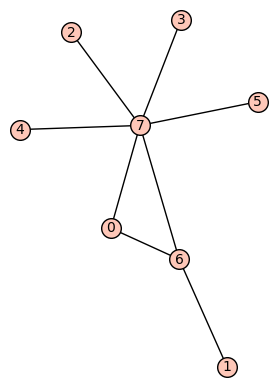
\includegraphics[height=5cm]{min_graf_8_1}
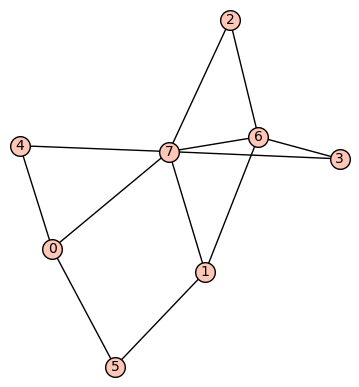
\includegraphics[height=5cm]{min_graf_8_2}
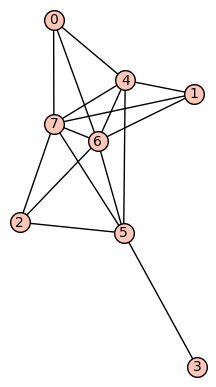
\includegraphics[height=5cm]{min_graf_8_3}
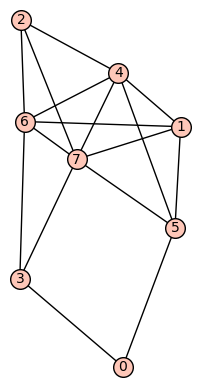
\includegraphics[height=5cm]{min_graf_8_4}
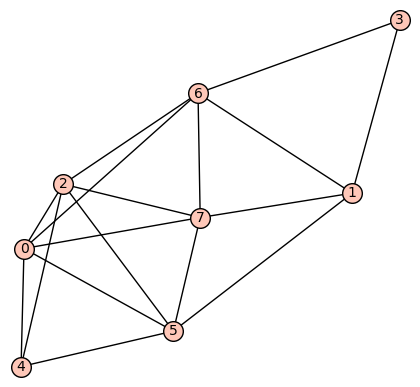
\includegraphics[height=5cm]{min_graf_8_5}
\end{center}

Za grafe na devetih vozliščih traja preverjanje že nekaj minut. Izmed vseh $261080$ generiranih grafov jih ima razliko $0$ natanko $46482$.

\begin{center}
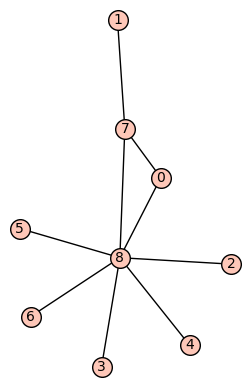
\includegraphics[height=5cm]{min_graf_9_1}
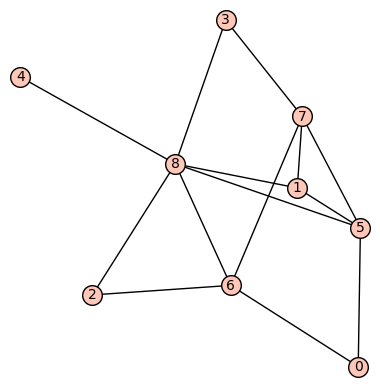
\includegraphics[height=5cm]{min_graf_9_2}
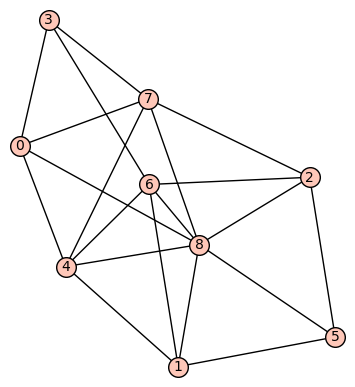
\includegraphics[height=5cm]{min_graf_9_3}
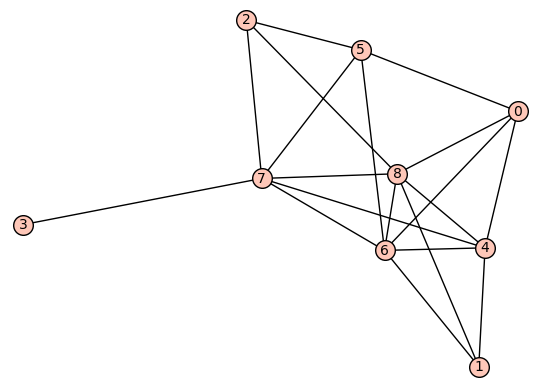
\includegraphics[height=5cm]{min_graf_9_4}
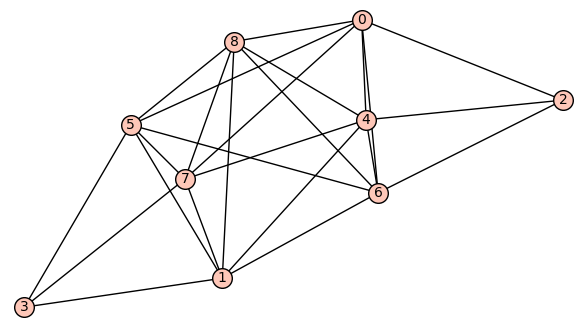
\includegraphics[height=5cm]{min_graf_9_5}
\end{center}

Grafe na desetih vozliščih program preverja nekoliko več kot $4$ ure. Generiranih je $11716571$ grafov in minimalna razlika je ponovno $0$, takih grafov je $2284660$.

\begin{center}
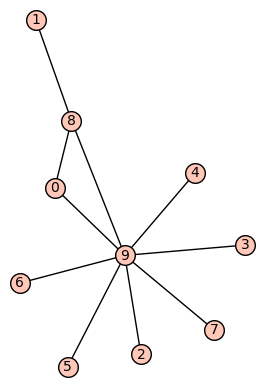
\includegraphics[height=5cm]{min_graf_10_1}
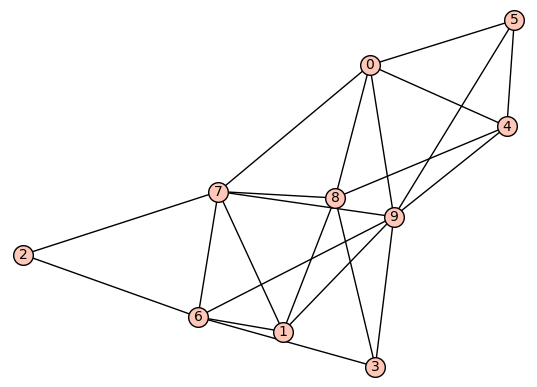
\includegraphics[height=5cm]{min_graf_10_2}
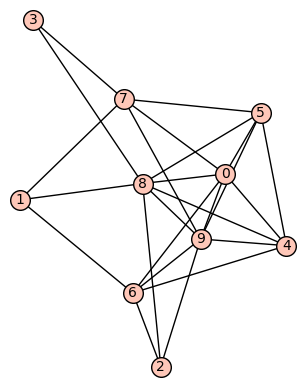
\includegraphics[height=5cm]{min_graf_10_3}
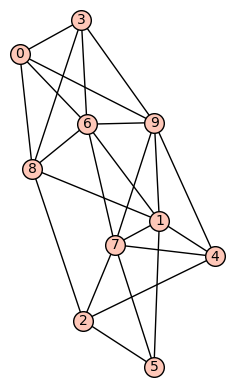
\includegraphics[height=5cm]{min_graf_10_4}
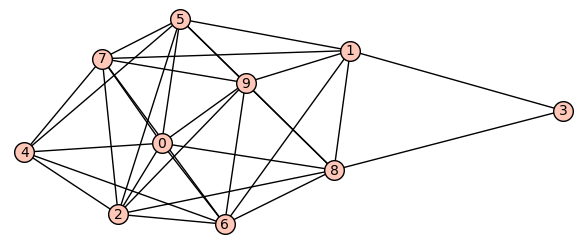
\includegraphics[height=5cm]{min_graf_10_5}
\end{center}

Zaključimo lahko, da dana domneva $Graffiti\ conjecture\ 232$ vsekakor velja na majhnih grafih z deset ali manj vozlišči.

\section{Veliki grafi}
Za velike grafe ($n\leq50$) sva uporabila vgrajeno funkcijo $graphs.RandomGNP(n,p)$. Ta funkcija generira graf z n vozlišči in ustvari povezavo med dvema vozliščema z verjetnostjo p. Funkcijo preverjanje domneve sva nekoliko modificirala in nato ustvarila generator grafov za vozlišča za $n=50,75,100$ in verjetnosti $p=0.33,0.5,0.66$. Vsako kombinacijo sva preverila 1000-krat. Tak program porabi približno 1 uro in 10 minut za izračun. Čas je bil izmerjen s pomočjo knjižnice $datetime$. Program je shranjeval najmanjšo razliko, ki jo je našel. Če je bila ta manjša ali enaka 2 je graf shranil v seznam $mala\_razlika$.

\begin{center}
\textbf{Preverjanje domneve za velike grafe}
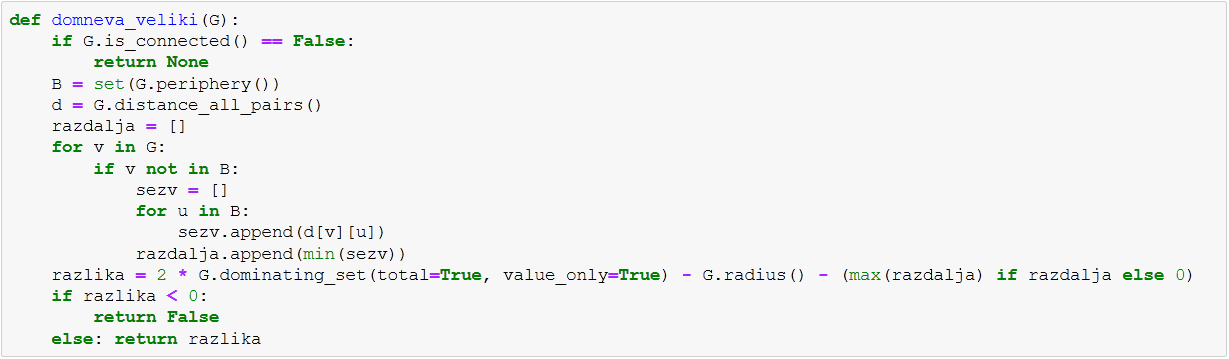
\includegraphics[width=16cm]{domneva_veliki}
\end{center}

\pagebreak

\begin{center}
\textbf{Generator velikih grafov}
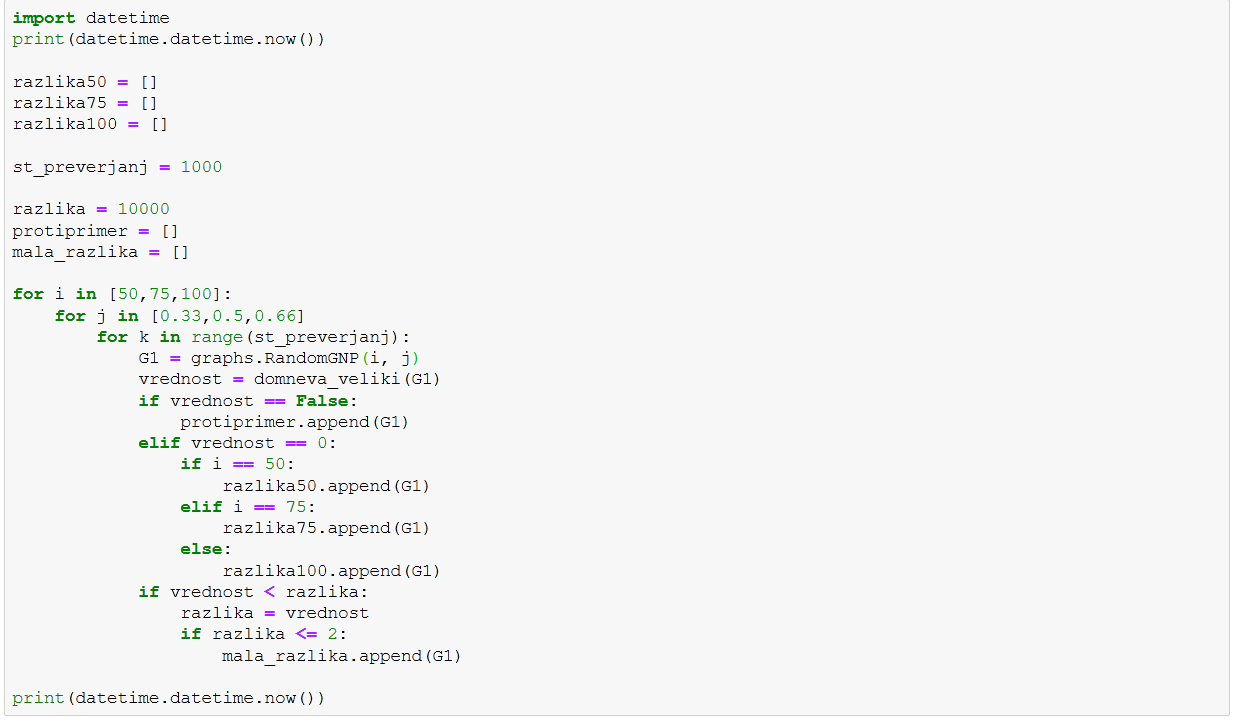
\includegraphics[width=16cm]{veliki_grafi}
\end{center}

Program sva pognala večkrat, v končnem sva preverila več kot 30000 grafov (ne nujno različnih). Nikoli se ni zgodilo, da bi obstajal protiprimer, še več razlika je bila vedno večja od 0. Pri grafih $n=50$ in $p=0.66$ se je pojavil primer, ko je bila razlika 2. To je najmanjša razlika, kar se jih je pojavilo pri generiranju.

\begin{center}
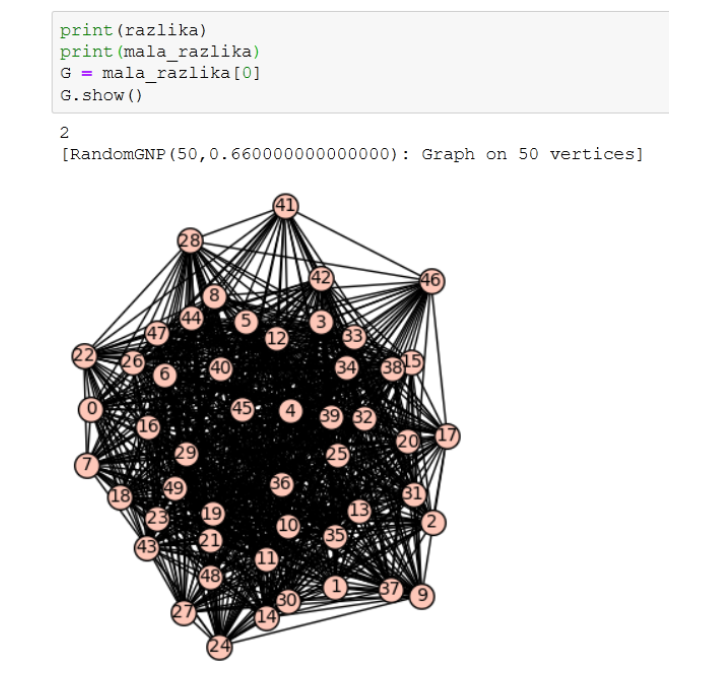
\includegraphics[height=8.5cm]{graf_razlika_2}
\end{center} 

Na koncu sva preverila še 3500 grafov z $n=200$ in $p=0.66$, kar je trajalo približno 5 ur. Razlika je bila 4, ta razlika je bila tudi najbolj pogosta pri vseh generiranjih.

\begin{center}
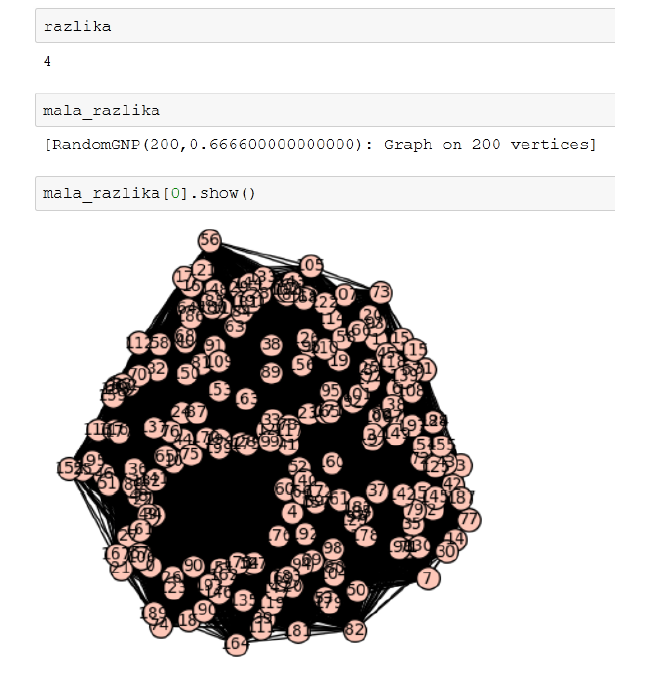
\includegraphics[height=8.5cm]{graf_200}
\end{center}

\subsection{Lokalno iskanje}
Po direktni analizi sva začela z local extrema search. Ideja je, da generiramo naključen graf z $n$ vozlišči, preverimo domnevo, nakar izberemo naključni vozlišči in dodamo povezavo, če ne obstaja oziroma odstranimo povezavo, če obstaja. Potem še enkrat preverimo domnevo na spremenjenem grafu, če je rezultat enak ali boljši (neenakost bližje 0) potem nadaljujemo na novem grafu, sicer odstranimo spremembo in ponovno izberemo naključni vozlišči. To nardimo za $k$ korakov nakar vrnemo graf in rezultat neenakosti domneve. V primeru, da bi našli protiprimer, program takoj konča in izpiše rezultat. S tem iščemo le lokalni ekstrem, ta je, če slučajno začnemo na pravem mestu, lahko tudi globalni.

Preverjala sva grafe velikosti 10 (rezultat 2), 20 (rezultat 2) in 50 (rezultat 2), kjer sva uporabljala število korakov $k=2000$. Izkazalo se je, da večje število korakov ni vračalo manjših rezultatov. Potem sva izvajala program še za 100 in 200 vozlišč. Že od prej vemo, da testiranje domneve na 200 vozliščih za 3500 grafov traja približno 5 ur. Zato sva število korakov zmanjšala na $k=700$ in s tem čas na 1 uro. Za 100 vozlišč pa 500 korakov traja približno 20 minut, torej 1500 traja približno 1 uro, zato $k=1500$. Verjetnost povezave med vozliščema pri generiranju grafa je bila $p=0.8$, saj sva pri direktni analizi dobivala boljše rezultate, kot pri manjših verjetnostih. Rezultati so bili boljši kot pri direktni analizi, saj sva tudi za $n=100,200$ našla primere, kjer je bila razlika enaka 2. Spodaj so navedeni primeri grafov kjer so bile razlike majhne, pri $n=10$ je 0, pri 15, 20, 100 pa je 2.

\begin{center}
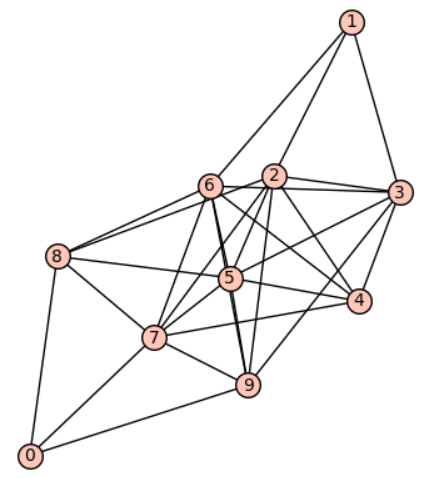
\includegraphics[width=5cm]{graf_10_0}
\end{center}

\begin{center}
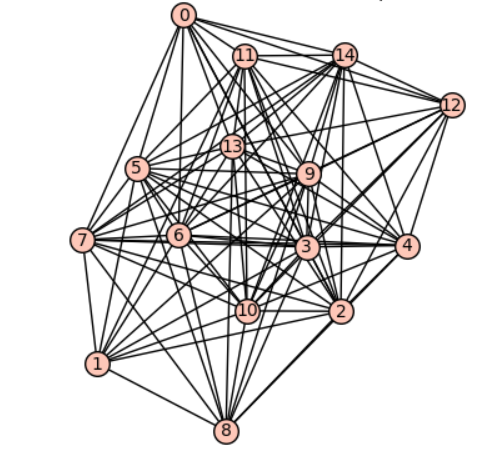
\includegraphics[width=6cm]{graf_15_2}
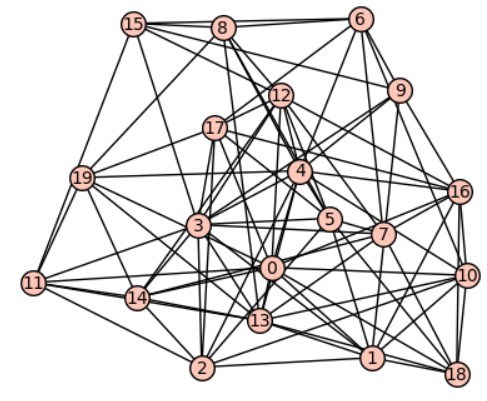
\includegraphics[width=6cm]{graf_20_2}
\end{center}

\begin{center}
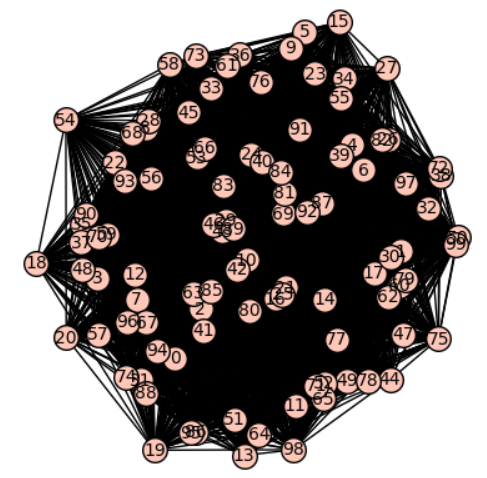
\includegraphics[width=6cm]{graf_100_2}
\end{center}

\subsection{Simulated Annealing}
Na koncu sva naredila še Simulated Annealing (SA) analizo. Ideja SA je predvsem, da je ocena globalnega ekstrema lahko boljša od točnega lokalnega. Točnega globalnega ekstrema zaradi časovne zahtevnosti ni moč izračunati.

\pagebreak

\subsubsection{Delovanje SA}
Vsako povezavo, ki razliko pri domnevi zmanjša dodamo/odstranimo z neko verjetnostjo. Torej vzamemo dve naključni vozlišči in kot prej dodamo/odstranimo povezavo, nakar preverimo domnevo in v primeru, da je razlika enaka ali manjša, z neko verjetnostjo nadaljujemo na tem novem grafu, sicer na starem. S tem se izognemo konvergenci v lokalen ekstrem. Še vedno izbiramo le boljše oziroma enake grafe, zato algoritem ne divergira. Algoritem, se torej od iskanja lokalnega ekstrema razlikuje v tem, da se, z dodatkom verjetnosti pri dodajanju/odstranjevanju povezav, izognemo konvergenci v lokalen ekstrem, ampak gremo proti globalnemu. 

Sedaj sva tudi za grafe velikosti do $n=50$ dobila rezultat 0 (prej le za $n=10$), a nikoli protiprimera. Za grafe do $n=25$ sva v najmanj 2000 korakih našla graf z rezultatom 0. Zanimivo je, da nama pri $n=50$ in $p=0.75$ ni uspelo najti rezultata manjšega od 2, pri $p=0.4$ pa je bil rezultat tudi 0, število korakov pa sva povečala na $k=150000$, kar je trajalo približno 1h.

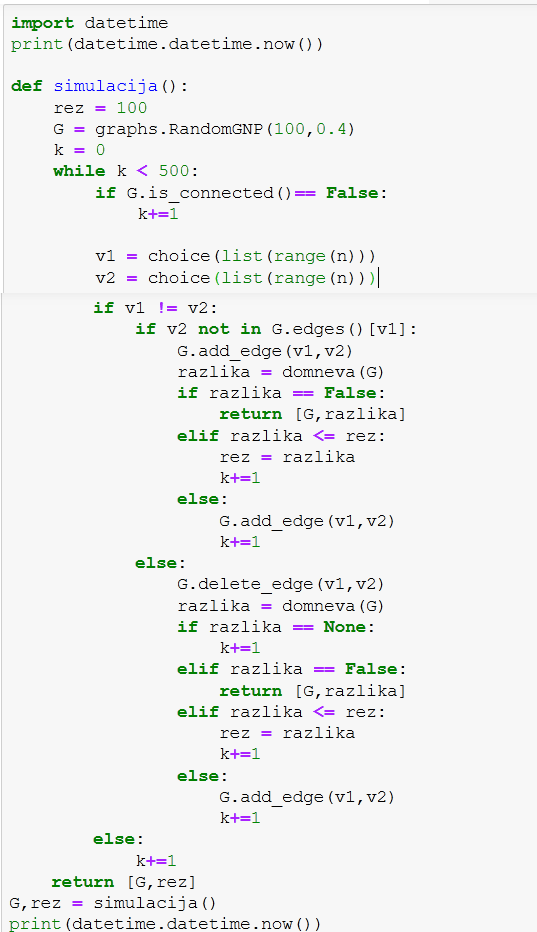
\includegraphics[scale=0.6]{Simulacija} 

\begin{center}
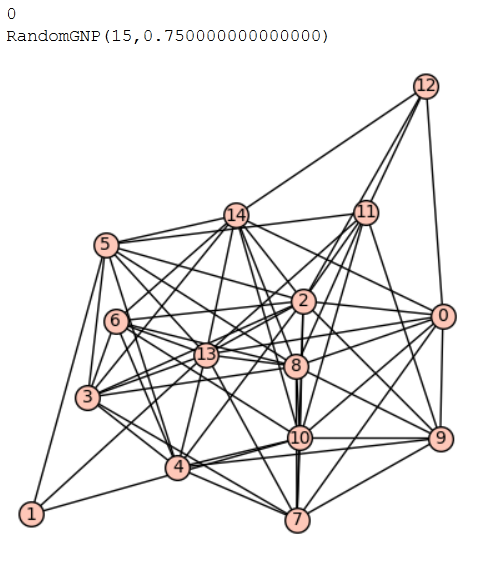
\includegraphics[width=6cm]{graf_15_0}
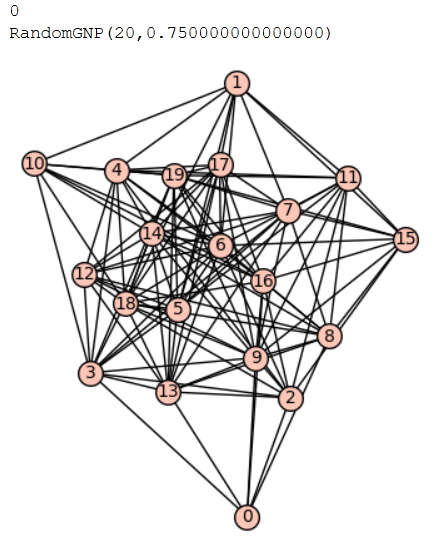
\includegraphics[width=6cm]{graf_20_0}
\end{center}

\begin{center}
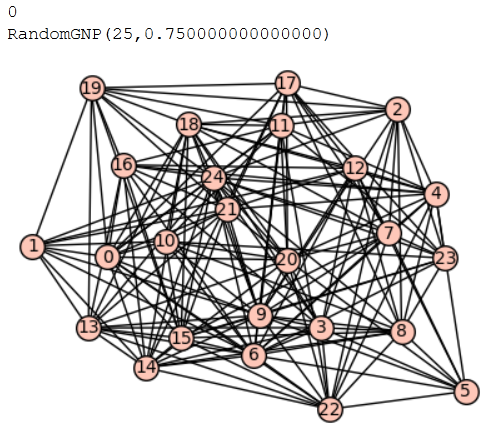
\includegraphics[width=6cm]{graf_25_0}
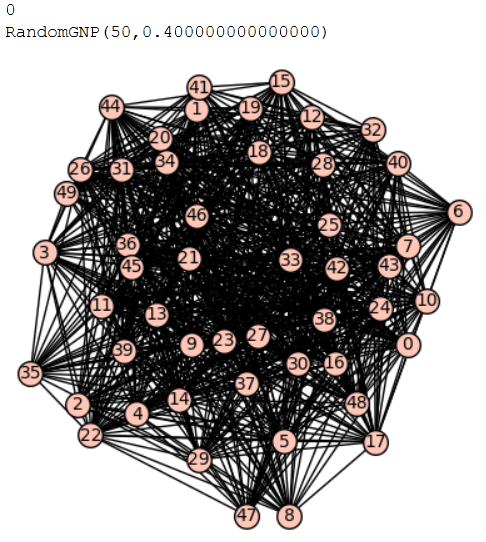
\includegraphics[width=6cm]{graf_50_0}
\end{center}

\end{document}